\documentclass{llncs}
\usepackage{times}
\usepackage[T1]{fontenc}
\usepackage[utf8]{inputenc}
\usepackage{aeguill}
\usepackage[portuguese]{babel}
\setcounter{secnumdepth}{3}

% Comentar para not MAC Users
%\usepackage[applemac]{inputenc}

\usepackage{a4}
%\usepackage[margin=3cm,nohead]{geometry}
\usepackage{epstopdf}
\usepackage{graphicx}
\usepackage{fancyvrb}
\usepackage{amsmath}
%\renewcommand{\baselinestretch}{1.5}


\begin{document}
\mainmatter
\title{TP2 : Balanceamento de Carga com servidor proxy invertido}

\titlerunning{TP2 : Balanceamento de Carga com servidor proxy invertido}

\author{Cesário Perneta \and Rui Rodrigues \and Tiago Fraga}

\authorrunning{Cesário Perneta \and Rui Rodrigues \and Tiago Fraga}

\institute{
University of Minho, Department of  Informatics, 4710-057 Braga, Portugal\\
e-mail: \{a73883,a74572,a74092\}@alunos.uminho.pt
}

\date{\today}
\bibliographystyle{splncs}

\maketitle
\begin{abstract}
Para muito serviços, um único servidor não é suficiente para dar vazão aos pedidos dos clientes. Nesses casos é necessário ter uma pool de servidores, com N servidores capazes de dar resposta aos pedidos. Ainda assim o serviço terá um único ponto de entrada para todos os clientes. Trata-se de um servidor de \textit{front-end}, com um nome e um endereço \textit{IP} únicos e bem conhecidos, cuja tarefa é atender às conexões dos clientes e desviá-las para um dos servidores de \textit{back-end} disponíveis. Esse servidor designa-se normalmente por \textit{Reverse Proxy}.	
\end{abstract}



\section{Introdução} \label{intro}

No presente relatório será abordado a resolução e verificação do segundo trabalho prático da unidade curricular de Comunicação por Computadores. Irá ser possivel encontrar uma análise detalhada do enunciado e das medidas que encontramos para o resolver, bem como, de todas as classes, funções e variáveis implementadas ao logo do projecto. Por fim, apresentamos alguns dos testes efetuados às aplicações criadas, de forma a entender todo o problema.
Com a realização deste trabalho prático o objectivo da equipa docente era a motivação dos alunos para a utilização da comunicação por sockets \textbf{UDP} e sockets \textbf{TCP}.
Numa primeira fase, tinhamos como objetivo implementar a \textbf{Tabela de Estado} onde é possivel guardar todas as informações de todos os \textbf{Agentes UDP} que tambem iam ser criados nesta primeira etapa. Além disto, temos de implementar o \textbf{Monitor UDP} que é a unidade principal da primeira parte do projecto, pois é ele, que faz a comunicação com os \textit{Agentes UDP} e atualizam a sua informação na \textit{Tabela de Estado}. Ainda nesta fase, foi nos proposto desenhar os \textit{Protocol Data Unit} - \textbf{PDU's}, que iam ser os objetos de comunicação dos \textit{Agentes UDP} com o \textit{MonitorUDP}. Por fim, foram realizados alguns testes, com o objetivo de verificar se esta fase estava a operar da maneira correta e era possivel prosseguir para a fase seguinte.
Numa segunda fase, temos de implementar o \textbf{Reverse Proxy}. Começamos por definir o algoritmo de seleção do \textbf{Web Server} onde os nossos \textit{Agentes UDP} estavam a operar, de seguida, implementamos o servidor que ia fazer a comunicação entre o \textbf{Browser} e o \textbf{Web Server} através de sockets TCP. Por fim, assim como na primeira etapa, foram realizados testes de forma a verificar a correta execução de toda a aplicação.


\section{Arquitetura da solução}


		\begin{enumerate}

			\item \textbf{Tabela Estado} - uma estrutura de dados partilhada, que mantém toda a informação necessária para o algoritmo de seleção de servidor poder funcionar. Nesta tabela é possivel encontrar: 
			\begin{itemize}
				\item{ID do Agente UDP;}
				\item{IP;}
				\item{Porta;}
				\item{ID da resposta ao ultimo request;}
				\item{RAM utilizada;}
				\item{CPU utilizado;}
				\item{URL do servidor Web que está a operar;}
			\end{itemize}
			\bigskip
			\item \textbf{AgenteUDP} - Este agente escuta pedidos de \textit{probing} na porta 8888 enviados pelo MonitorUDP por multicast para o grupo Multicast com endereço \textit{IPv4 239.8.8.8}. Antes de ficar à escuta em UDP na porta 8888 o agente junta-se ao grupo multicast referido. Por cada mensagem recebida, o agente cria uma resposta com uma mensagem UDP dirigida em unicast ao MonitorUDP, onde é incluindo na resposta todos os pontos descritos no ponto 1.

			\bigskip
			\item \textbf{MonitorUDP} - É um agente UDP responsável pela descoberta de servidores, no nosso caso definimos que de 10 em 10 segundos envia uma mensagem de \textit{probing}, por UDP, dirigida ao grupo Multicast 239.8.8.8 para a porta 8888.Escuta respostas UDP unicast na mesma porta e verifica a integridade de todas as mensagens recebidas antes de atualizar a TabelaEstado em conformidade.

			\bigskip
			\item \textbf{ReverseProxy} - Pertence ao monitorUDP, no entanto é um agente TCP capaz de atender pedidos na porta 80, vindos de qualquer cliente. A cada pedido recebido consulta a TabelaEstado, escolhe um dos servidores disponíveis usando um algoritmo de seleção e abre uma conexão TCP para o servidor escolhido. Todos os dados recebidos do cliente serão enviados de forma totalmente transparente (sem nenhum processamento, nem nenhum pressuposto) para o servidor e vice-versa. A conexão é terminada depois do servidor Web enviar a resposta ao cliente.

		\end{enumerate}

		\begin{figure}[h!]
		\centering
		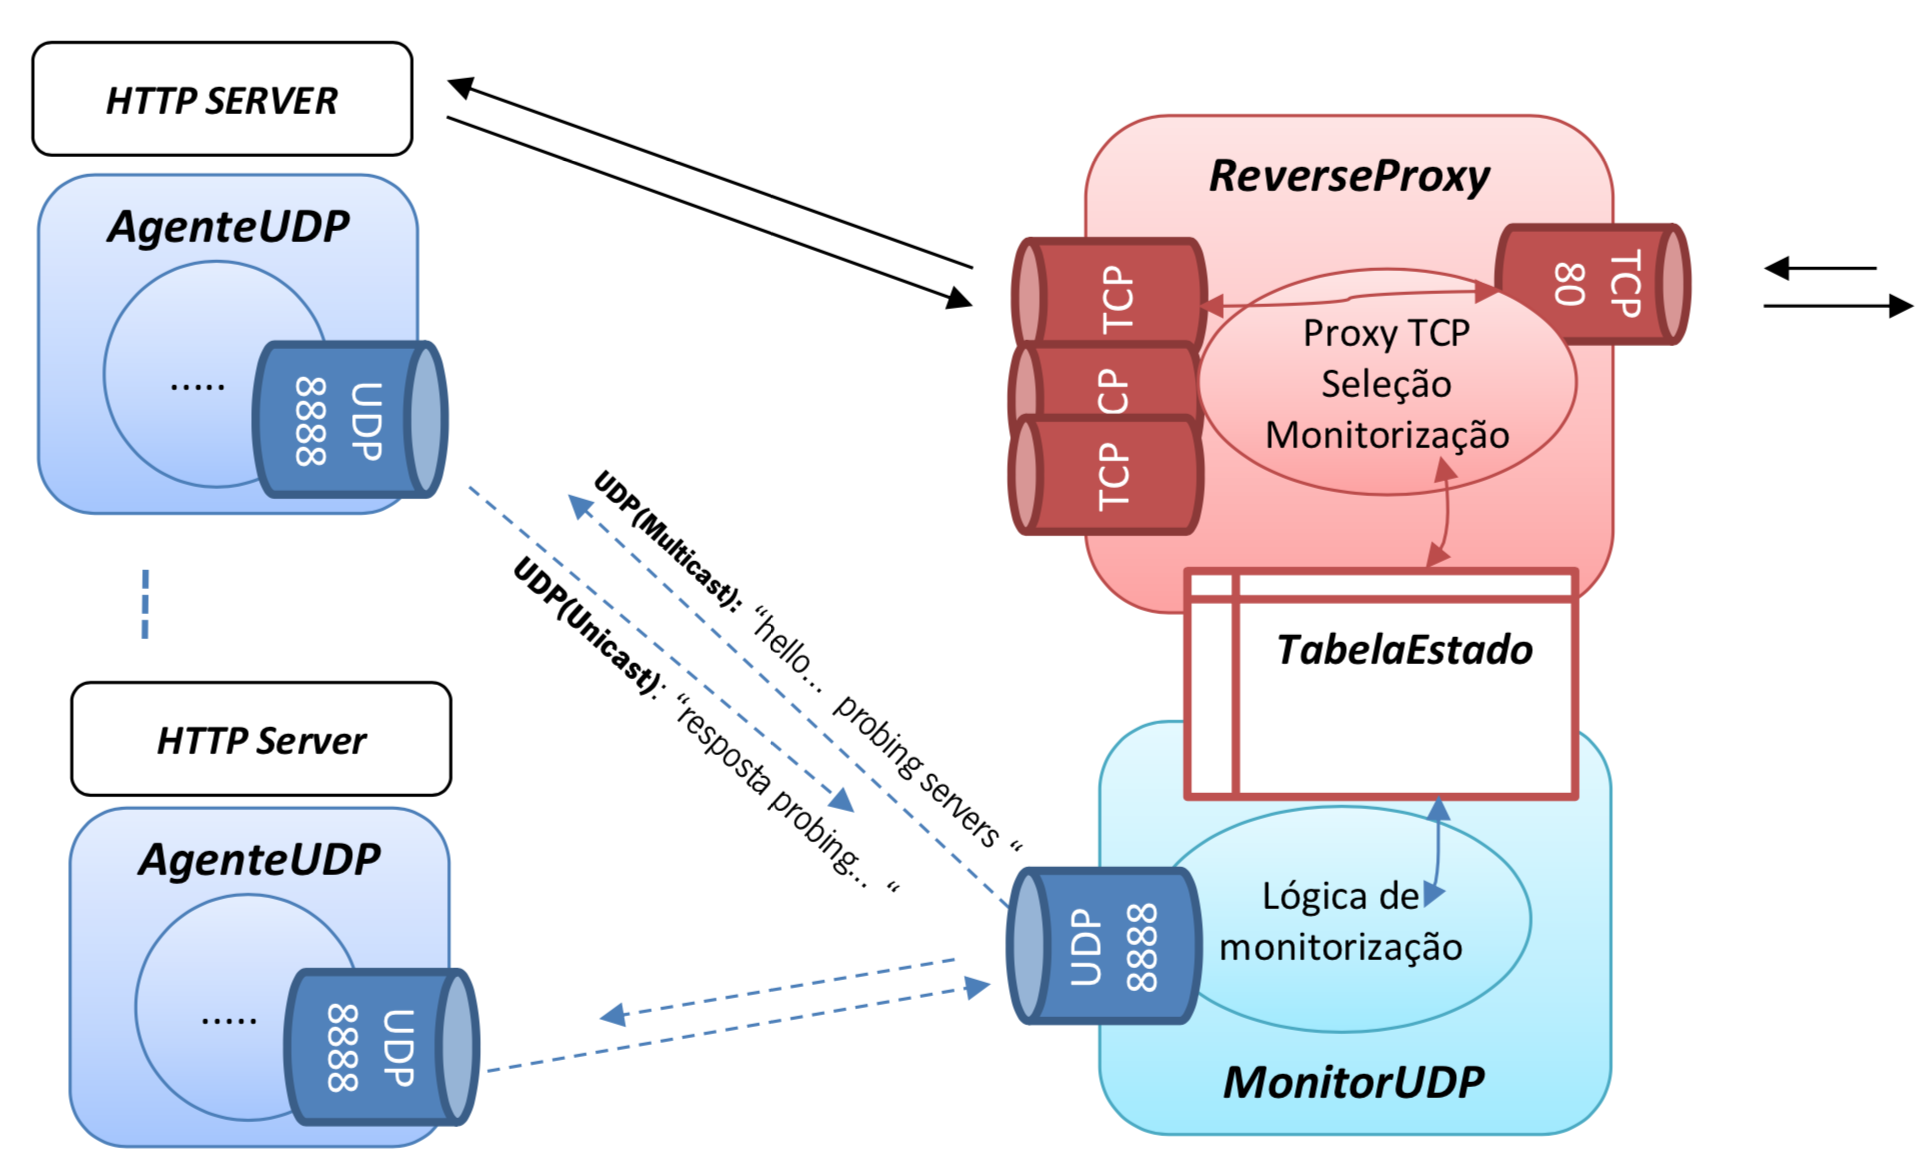
\includegraphics[scale=0.3]{figura1} 
		\caption{Arquitetura da Solução}
		\end{figure} 



\section{Especificação do protocolo UDP}

	\subsection{Formato das mensagens Protocolares (PDU)}

		\subsubsection{PDU de Envio - Probe Request} \

			Para definir o formato do \textit{Protocol Data Unit} de envio do monitorUDP para os agenteUDP concordamos que esta devia ter dois parametros importantes:

				\begin{enumerate}

					\item \textbf{ID} - Número que identifica a mensagem. Assim que o monitorUDP é ligado, este valor começa a zero e é iterado a cada vez que é enviado um pedido de probing, com o intuito de associar as respostas dos agentesUDP às mensagens enviadas.

					\item \textbf{MSG} - É o conteúdo da mensagem a enviar, no nosso caso vai ser uma simples frase a pedir um pedido de probing dos agentesUDP.

				\end{enumerate}

			No momento de ser enviado este pdu é convertido para o formato de \textbf{string}.

		\subsubsection{PDU de Resposta} 

			De forma a definir as \textit{Protocal Data Unit} de responsta dos agentesUDP para o monitorUDP tivemos de ter em atenção que temos de incluir na mensagem todos os parâmetros necessários para preencher a informação do agente na tabela de estado, como tal decidimos incluir os seguintes parâmetros no pdu de reposta: 

				\begin{enumerate}

					\item \textbf{NR} - É o numero que identifica a resposta com o pdu de probe.

					\item \textbf{ID} - É o numero que identifica o agenteUDP.

					\item \textbf{CPU} - É o valor de cpu gasto pelo agenteUDP.

					\item \textbf{MEMORY} - É o valor de memoria gasta pelo agenteUDP.

					\item \textbf{URL} - É o url do servidor \textit{Web} onde o agenteUDP está a operar.

				\end{enumerate}

			Assim como o pdu de probe, este pdu no momento do envio é convertido para o formato de \textbf{string}.

	\subsection{Interações}

		Com o intuito de perceber como funciona a troca de mensagens através de sockets UDP estudamos isoladamente o funcionamento das mensagens UDP entre um servidor e um cliente simples. Percebemos que este modo de trocar infornmação tinha algumas particulares diferenças em relação aos sockets que tinhamos estudado anteriormente noutras unidades curriculares, nomeadamente os sockets \textbf{TCP}.

		De forma a efetuar a interação entre os agentesUDP e o monitorUDP deve-se converter a mensagem a enviar no conjunto de bytes que ela ocupa, de forma a serem colocados num pacote de dados que por fim é enviado pelo canalUDP. Através do estudo descrito em cima, percebemos que teriamos de utilizar um socket especificio para os agentes se puderem juntar a um grupo em multicast - \textbf{Multicast Socket} - de forma a cria-lo apenas temos de especificar a porta onde vai operar e junta-lo ao grupo multicast pretendido através o endereço correspondente. Se pretendermos enviar dados em unicast temos de utilizar outro tipo de socket especifico - o \textbf{Datagram Socket}.

		As mensagens trocadas através dos sockets TCP são feitas de um modo que ja conheciamos, pois nao é preciso converter a mensagem em bytes, podendo ser enviada sem qualquer tipo de processamento através dos canaisTCP. Este tipo de interação só vai ser efetuado ao nivel do reverseProxy, isto é, entre o browser e o servidor web.




\section{Implementação}
	
	\subsection{Bibliotecas de funções}

		Fazendo uma análise pelo código implementado é possivel destacar o seguinte conjunto de bibliotecas de funções que foram utilizadas:

			\begin{enumerate}

				\item \textbf{java.net.MulticastSocket} - As funções utilizadas desta biblioteca, foram necessárias para conseguir fazer a correta implementação dos agentesUDP. Sem estas funções nao era possivel colocar cada agente à espera de pedidos probing num grupo UDP de multicast.
				\bigskip
				\item \textbf{java.net.DatagramSocket} e \textbf{java.net.DatagramPacket} - Utilizamos as funções destas bibliotecas para criar corretamente os socketsUDP e os correspondentes \textit{packets} para fazer a troca de informação através de sockets UDP.
				\bigskip
				\item \textbf{java.net.InetAddress} - Esta biblioteca foi usada para obter o endereço dos agentesUDP depois destes enviarem os pdu's de resposta para o monitor.
				\bigskip
				\item \textbf{java.lang.management.ManagementFactory e com.sun.management.ThreadMXBean} - As funções destas duas bibliotecas foram utilizadas com o intuito de obter a quantidade de cpu e memoria ram gastos pelos agentesUDP.
				\bigskip
				\item \textbf{import java.net.ServerSocket e import java.net.Socket} - Estas duas bibliotecas serviram para a correta criação e manuseamento dos sockets TCP.
				\bigskip
				\item \textbf{import java.net.HttpURLConnection e import java.net.URL} - Utilizamos estas bibliotecas de forma a fazer os pedidos de \textbf{GET} aos servidores web. 
				\bigskip
				\item \textbf{import java.io.File, import java.io.FileWriter e import java.awt.Desktop} - Estas três bibliotecas foram utilizadas com o intuito de criar um ficheiro html com a resposta dos servidores web ao pedido de \textit{GET} e, por fim, abri-lo no browser.
				\bigskip
				\item \textbf{outras} - Por último foram utilizadas bibliotecas de funções de forma a auxiliar a leitura da informação quer fosse do \textit{standar input} ou entao dos sockets.


			\end{enumerate} 

	\subsection{Classes implementadas}

		Após fazermos uma breve descrição de todas as bibliotecas que foram importadas para o nosso projecto de forma a auxiliar-nos na boa implementação do trabalho, vamos abordar detalhadamente as classes que desenvolvemos:

			\begin{enumerate}

				\item \textbf{AgenteUDP.java} - Esta é a classe onde está implementado todo o código referente aos agentesUDP. Depois de ser feito o registo inicial de cada agente com a introdução do seu identificador numerico, e do url do servidor web onde o agenteUDP vai estar a operar, este junta-se ao grupo multicast definido no seu construtor. Em seguida, entra num ciclo infinito, pois o agente deve estar constantemente a trabalhar e fica a espera de receber pedidos de probing no grupo multicast, posto isto, é feito o processamento da mensagem e é calculado a quantidade de cpu e ram gastos pelo agente. Por fim, é enviado o pdu de resposta ao monitor com todos os dados obtidos. As variáveis de instância desta classe são:
					\begin{itemize}
						\item{int id;} - id do agente;
						\item{String url;} - url do servidor web;
						\item{int port;} - porta do grupo multicast;
						\item{InetAddress endereco;} - endereço do grupo multicast;
						\item{long tempo;} - tempo de cada mensagem recebida. Nota: nao foi utilizado;
						\item{long cpu;} - cpu gasto pelo agente;
						\item{long memory;} - memoria ram gasta pelo agente;
					\end{itemize}

				\bigskip
				\item \textbf{InfoServidor.java} - Esta classe é onde está implementado todo o código referente aos objetos que são guardados na tabela de estado e armazenam a informação dos agentesUDP, ou seja, a nossa tabela de estado é um HashMap em que a key é o numero do agenteUDP e o value é um objeto do tipo \textbf{InfoServidor}, portanto é dentro deste objeto que guardados os dados de cada agenteUDP. Nesta classe apenas temos os métodos get/set e construtor. As variáveis de instância da classe são:
					\begin{itemize}
						\item{int lastProbe;} - numero da ultimo pedido probe a que o agente respondeu;
						\item{String url;} - url do servidor web;
						\item{InetAddress ip;} - endereço ip do agente;
						\item{int porta;} - porta UDP que o agente estava a utilizar;
						\item{long cpu;} - cpu gasto pelo agente;
						\item{long ram;} - memoria ram gasta pelo agente;
						\item{long rtt;} - rtt do agente;
					\end{itemize}


				\bigskip
				\item \textbf{MonitorUDP.java} - Esta classe é onde está implementado o código referente ao monitorUDP, nela está contida, um método de \textit{main}, como tal é um executável. Quando se inicia o monitor, são imediatamente criadas mais duas threads uma que vai tratar do código do reverseProxy, enquanto que outra vai tratar do código do monitorUDP\_Receiver. Ambas vão ser explicadas a seguir. Após este passo, e do socket UDP já estar criado o monitor entra num ciclo infinito, pois como os agentes é preciso estar constantemente a trabalhar, e é enviado o primeiro pdu request, de seguida a thread é adormecida durante 10 segundos e volta a repetir o ciclo até o monitor ser desligado pelo utilizador. De salientar que nesta classe está definido um método que imprime a tabela de estado a cada dez segundos como medida de teste dos resultados. As variáveis de instância da classe são:
					\begin{itemize}
						\item{HashMap<Integer,InfoServidor> tabela;} - tabela de estado do monitor
						\item{InetAdress endereco;} - endereço do grupo multicast
						\item{int port;} - porta do grupo multicast
						\item{long tempo;} - tempo de intervalo dos pdu de request
					\end{itemize}

				\bigskip
				\item \textbf{MonitorUDP\_Receiver.java} - Esta é a classe onde está implementado o código referente ao receiver do monitorUDP, ou seja, a thread que trata das respostas dos agentesUDP. Como esta classe é uma \textit{Runnable} vai ser implementado o seu método \textit{run}. Quando a thread é iniciada, é criado o socket UDP na porta que vai receber as repostas em unicast, e entra num ciclo infinito a aguardar a receção de mensagens. Quando recebe uma mensagem, é feito o seu processamento, para se perceber que dados foram enviados para posteriormente serem guardados na tabela de estado.
				A unica variavél de instancia desta classe é o objeto MonitorUDP onde foi criada a thread.

				\bigskip
				\item \textbf{PDUProbe.java} - Esta é a classe onde está o código do objeto onde é criado o pdu de probe do monitor. Apenas tem os métodos de get/set e construtor. As variáveis de instãncia da classe são:
					\begin{itemize}
						\item{int id;} - numero do probe;
						\item{String msg;} - mensagem probe a enviar;
					\end{itemize}

				\bigskip
				\item \textbf{PDUResponse.java} - Esta é a classe onde está o código do objeto onde é criado o pdu de resposta do agente. Apenas tem os métodos de get/set e construtor. As variáveis de instãncia da classe são:
					\begin{itemize}
						\item{int nr;} - numero do probe;
						\item{int id;} - numero do agente;
						\item{long cpu} - cpu gasta pelo agente; 
						\item{long memory} - memoria ram gasta pelo agente;
						\item{String url} - url do servidor web onde o agente está a operar;
					\end{itemize}

				\bigskip
				\item \textbf{ReverseProxy.java} - Esta é a classe onde está o código referente ao reverseProxy. Como esta classe é uma \textit{Runnable} vai ser implementado o seu método \textit{run}. Quando a thread é iniciada, é criado o socket TCP de servidor e este fica a espera de conexões num ciclo infinito. Quando recebe um pedido de conexão é criada uma thread para tratar dessa conexão. Nesta classe está implementado o método que faz a escolha do servidor web para onde deve ser desviado o pedido do cliente. O servidor web escolhido é o que tem os valores de cpu e ram utilizados mais baixos.
				As variávies de instância desta classe são:
					\begin{itemize}
						\item{HashMap<Integer,InfoServidor> tabela;} - a tabela de estado;
						\item{int port;} - a porta onde vai esperar por conexões;
						\item{ServerSocket serverSocket;} - servidor TCP;
					\end{itemize}

				\bigskip
				\item \textbf{Server\_Worker.java} - Esta é a classe onde está o código referente ao worker do reverseProxy, nela são tratados os pedidos de conexão. Como esta classe é uma \textit{Runnable} vai ser implementado o seu método \textit{run}. Quando a thread é iniciada, é feita a escolha do servidor através do métoo referido no ponto anterior, de seguida é feito o pedido \textbf{GET} ao servidor onde o agente escolhido está a operar. Por fim, a resposta do servidor web é enviada pelo socket TCP sem qualquer tipo de processamento e a thread termina a sua execução. As variáveis de instância da classe são:
					\begin{itemize}
						\item{ReverseProxy proxy} - objeto reverseProxy que criou a thread;
						\item{Socket socket;} - socket que comunica com o cliente;
						\item{BufferedWriter out}
					\end{itemize}

				\bigskip
				\item \textbf{Cliente.java} - Esta é uma classe onde está o código referente a um cliente teste, que faz um pedido de conexão ao reverse proxy. Apenas faz o pedido de conexão ao reverse proxy, e recebe a resposta do pedido, cria um ficheiro html com ela e abre-a no browser.
			
			\end{enumerate}

\section{Testes e Resultados}

	Após ser feitos alguns testes, é possivel observar que todo o trabalho está a funcionar corretamente. Em relação à primeira parte, a troca de informação entre os agentes e o monitor é comprovada através da impressão da tabela de estado depois de cada pedido de probing ser enviado, como tal podemos constatar que funciona exatamente como nos foi pedido. Na segunda parte, não executamos os testes como nos foi pedido pelo professor, visto que temos os agentesUDP a operar na nossa máquina e enviar pedidos \textit{GET} para servidores externos e os pedidos de conexão serem simulados por um cliente em java e não pelo browser. Apesar destas diferenças os resultados obtidos são os mesmos dos que eram esperados pela forma inicialmente pedida. Fizemos esta pequena alteração apenas para ter mais facilidade no momento de executar os testes e desta forma poupar algum tempo na implementação do projeto.

\section{Conclusão} \label{concl}

	Dado por terminado o segundo trabalho prático da unidade curricular de Comunicação por Computadores, podemos concluir que o projeto desenvolvido é um autêntico sucesso.
	A realização deste trabalho foi um bom modo de familiarizar e aprender o funcionamento de troca de informação com o auxilio de sockets UDP e o funcionamento de um reverse proxy com uma pool de servidores.
	A principal dificuldade que encontramos, foi a de, numa primeira fase, perceber como íamos implementar os sockets UDP, e numa segunda fase, perceber como íamos executar os pedidos de \textit{GET} aos servidores web. Ultrapassadas estas dificuldades, prosseguimos para a elaboração de um trabalho fiável, robusto e competente.
	Deste modo, através do trabalho realizado e dos testes efetuados, podemos afirmar que o nosso projecto é capaz de implementar um Reverse Proxy de uma pool de servidores.










\end{document}
